\documentclass[runningheads,a4paper]{llncs}
\usepackage[utf8]{inputenc}
% linewrap symbol
\usepackage{color}
\definecolor{grey}{RGB}{160,160,160}
\newcommand{\linewrap}{\raisebox{-.6ex}{\textcolor{grey}{$\hookleftarrow$}}}

% proper encoding
\usepackage[T1]{fontenc}

\usepackage{flushend}
\usepackage{verbatim} 

\usepackage{textcomp}
\usepackage{listings}
\lstset{frame=lines,captionpos=b,numberbychapter=false,escapechar=§,basicstyle=\ttfamily,upquote=true}

% todo macro
\usepackage{color}
\newcommand{\todo}[1]{\noindent\textcolor{red}{{\bf \{ToDo }#1{\bf \}}}}

\usepackage{times}
%\usepackage{epsfig}
\usepackage{graphicx}
\usepackage{amsmath}
\usepackage{amssymb}
\usepackage{subfig}

% Thanks, http://lenaherrmann.net/2010/05/20/javascript-syntax-highlighting-in-the-latex-listings-package
\usepackage{color}
\definecolor{darkgray}{rgb}{.4,.4,.4}

\lstdefinelanguage{JavaScript}{
  keywords={push, typeof, new, true, false, catch, function, return, null, catch, switch, var, if, in, while, do, else, case, break},
  keywordstyle=\bfseries,
  ndkeywords={class, export, boolean, throw, implements, import, this},
  ndkeywordstyle=\color{darkgray}\bfseries,
  identifierstyle=\color{black},
  sensitive=false,
  comment=[l]{//},
  morecomment=[s]{/*}{*/},
  commentstyle=\color{darkgray},
  stringstyle=\color{red},
  morestring=[b]',
  morestring=[b]"
}

% If you comment hyperref and then uncomment it, you should delete
% egpaper.aux before re-running latex.  (Or just hit 'q' on the first latex
% run, let it finish, and you should be clear).
\usepackage{hyperref}
\def\sectionautorefname{Section}

\begin{document}

\mainmatter

\title{Crowdsourcing Event Detection in YouTube Videos}

% a short form should be given in case it is too long for the running head
\titlerunning{Crowdsourcing Event Detection in YouTube Videos}

% the name(s) of the author(s) follow(s) next
%
% NB: Chinese authors should write their first names(s) in front of
% their surnames. This ensures that the names appear correctly in
% the running heads and the author index.
%
\author{Thomas Steiner$^{1}$ \and Ruben Verborgh$^{2}$ \and Rik Van de Walle$^{2}$ \and \\Michael Hausenblas$^{3}$ \and Joaquim Gabarr\'{o} Vall\'{e}s$^{1}$}
\institute{Universitat Polit\'ecnica de Catalunya -- Department LSI\\
08034 Barcelona, Spain\\
\urldef{\emails}\path|{tsteiner,gabarro}@lsi.upc.edu|\emails
\and Ghent University -- IBBT, ELIS -- Multimedia Lab\\Gaston Crommenlaan 8 bus 201, B-9050 Ledeberg-Ghent, Belgium\\
\urldef{\emails}\path|{ruben.verborgh,rik.vandewalle}@ugent.be|\emails
\and DERI, NUI Galway IDA Business Park, Lower Dangan Galway, Ireland\\
\urldef{\emails}\path|michael.hausenblas@deri.org|\emails
}
%
\authorrunning{Crowdsourcing Event Detection in YouTube Videos}
% (feature abused for this document to repeat the title also on left hand pages)

\maketitle
% \thispagestyle{empty}

%%%%%%%%% ABSTRACT
\begin{abstract}
Considerable efforts have been put into making video content on the Web more accessible, searchable, and navigable by research on both textual and visual analysis of the actual video content and the accompanying metadata. Nevertheless, most of the time, videos are opaque objects in websites. With Web browsers gaining more support for the HTML5 \texttt{<video>} element, videos are becoming first class citizens on the Web. In this paper we show how events can be detected on-the-fly through crowdsourcing (i) textual, (ii) visual, and (iii) behavioral analysis in YouTube videos, at scale. The main contribution of this paper is a generic crowdsourcing framework for automatic and scalable semantic annotations of HTML5 videos. Eventually, we present our preliminary results using traditional server-based approaches to video event detection as a baseline. 
\end{abstract}

%%%%%%%%% BODY TEXT
\section{Introduction}
Official statistics~\cite{youtube:stats} from YouTube---owned by Google and one of the biggest online video platforms---state that more than 13 million hours of video were uploaded during~2010, and that 48~hours of video are uploaded every single minute. Given this huge and ever increasing amount of video content, it becomes evident that advanced search techniques are necessary in order to retrieve the few needles from the giant haystack. Closed captions allow for keyword-based in-video search, a feature announced \linebreak in 2008~\cite{googlevideo}. Searching for a phrase like \emph{``that's a tremendous gift''}, a caption from Randy Pausch's famous last lecture titled \emph{Achieving Your Childhood Dreams}~\footnote{\url{http://www.youtube.com/watch?v=ji5\_MqicxSo}}, indeed reveals a link to that lecture on YouTube. If no closed captions are available, nor can be automatically generated~\cite{youtubecaptions}, keyword-based search is still available over tags, video descriptions, and titles. Presented with a potentially huge list of results, preview thumbnails based on video still frames help users decide on the most promising result.

A query for---at time of writing---recent events such as the London riots\footnote{\url{http://en.wikipedia.org/wiki/2011_London_riots}} or the shooting in Ut\o ya\footnote{\url{http://en.wikipedia.org/wiki/2011_Norway_attacks}} reveals a broad selection of all sorts of video content, either professionally produced or, more often, shaky amateur videos taken with smartphones. Despite these and other differences, their thumbnails are typically very similar, as can be seen in~\autoref{fig:thumbnails}. These thumbnails are automatically generated by an unpublished computer vision-based algorithm~\cite{googleresearch}. From a user's point of view, it would be very interesting to see whether a video contains different shots. For example, a back-and-forth between a news anchorman and live images can be an indicator for professionally  produced content, whereas a single shot covering the entire video can be an indicator for amateur-generated eyewitness footage.

\begin{figure}[htb!]
  \begin{center}
   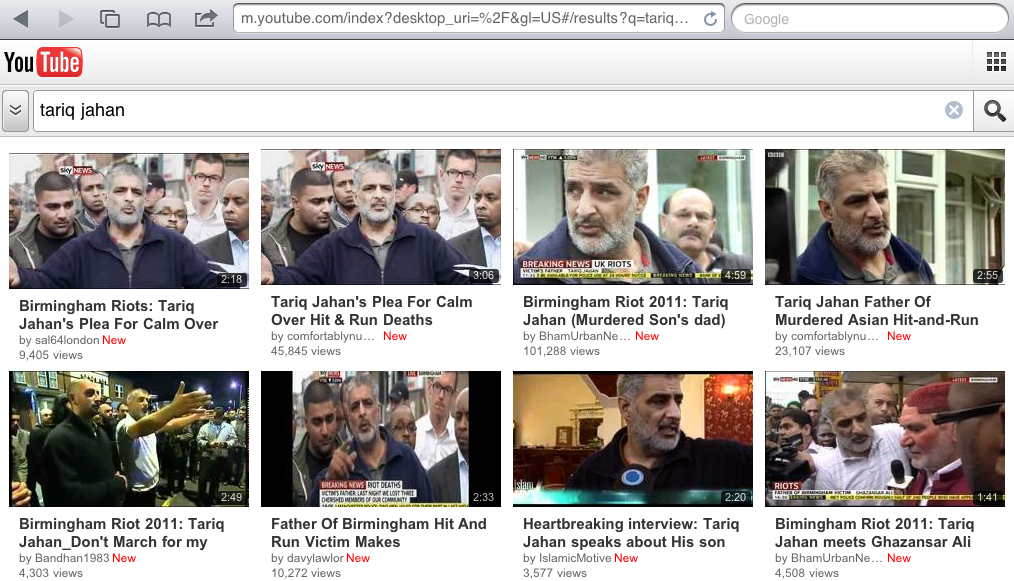
\includegraphics[width=0.7\linewidth]{./resources/tariq}
  \end{center}  
  \caption{YouTube search for ``tariq jahan'', father of a victim of the London riots.}
  \label{fig:thumbnails}
\end{figure}

In addition to the information provided by the separation of a video in shots, listing occurrences of named entities and their disambiguation can help users quickly decide whether a given video is of interest. For example, if a video about Ut\o ya contains an occurrence of the Norwegian Prime Minister Jens Stoltenberg, or a video about the London riots contains an occurrence of the Prime Minister of the United Kingdom David Cameron, they can potentially be considered more trustworthy than other videos. It is up to the user to judge the trustworthiness aspect, however, the more context is available, the easier this decision gets.

While the detection of persons and their identification would be possible through face detection and face recognition techniques, this task is computationally expensive. As we have shown in~\cite{semwebvid}, however, good results are possible through the analysis of the available textual metadata with Natural Language Processing (NLP) techniques, especially given the availability of (possibly automatically generated~\cite{youtubecaptions}) closed captions on YouTube. Finally, for videos that are longer than the attention span of a typical YouTube user, exploiting purposeful in-video navigation data can help determine points of interest within videos. For example, many users might skip the intros typically contained in professionally produced video content, or jump to spectacular shots directly. 

We define three types of events: \emph{visual events} in the sense of shot changes, \emph{occurrence events} in the sense of the appearance of a named entity, and \emph{interest-based events} in the sense of purposeful in-video navigation by users. In this paper, we report on a~browser extension that enables crowdsourcing  of event detection in YouTube videos through a combination of \emph{textual}, \emph{visual}, and \emph{behavioral} analysis techniques. When a~user starts watching a video, three processes start:

\paragraph{Visual Events}
We detect shots in the video by visually analyzing its content. We do this with the help of a browser extension, i.e., the whole process runs on the client-side using the modern HTML5~\cite{w3c_html5} JavaScript APIs of the \texttt{<video>} and \texttt{<canvas>} elements. As soon as the shots have been detected, we offer the user the choice to quickly jump into a specific shot by clicking on a representative still frame. 

\paragraph{Occurrence Events}
We analyze the available video metadata using NLP techniques, as outlined in~\cite{semwebvid}. The detected named entities are presented to the user in a list, and upon click via a timeline-like user interface allow for jumping into one of the shots where the entity occurs.

\paragraph{Interest-based Events} As soon as the \emph{visual events} have been detected, we attach JavaScript event listeners to each of the shots and count clicks on shots as an expression of interest in those shots.
 
\autoref{fig:youtube} shows the seamless integration of the detected events into the YouTube homepage. Contributions of this paper are the browser extension itself as well as the underlying crowdsourcing framework for automatic and scalable semantic annotations of HTML5 videos.

\begin{figure}[htb!]
\begin{center}
   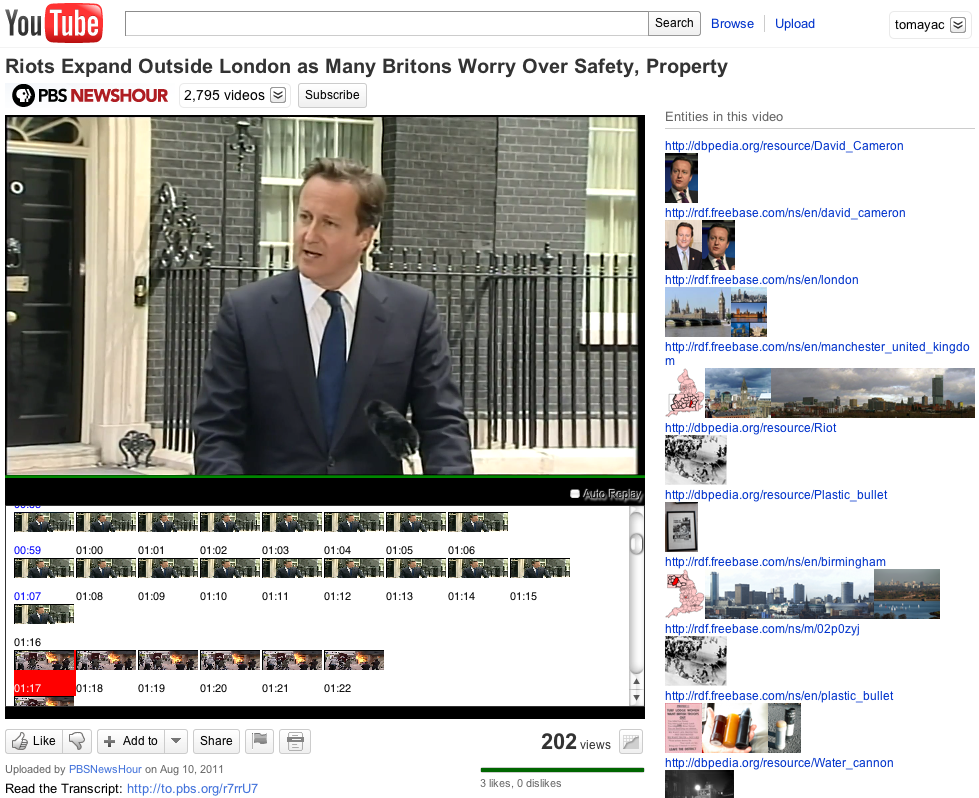
\includegraphics[width=0.8\linewidth]{./resources/youtube}
\end{center}
   \caption{Screenshot of the YouTube browser extension, showing the three different event types: \emph{visual events} (video shots below the video), \emph{occurrence events} (contained named entities and their depiction at the right of the video), and \emph{interest-based events} (points of interest in the video highlighted with a red background in the bottom left).}
\label{fig:youtube}
\end{figure}

\section{Related Work} \label{sec:related-work}
Many different approaches to event detection in video exist.
A~first category is artificial vision, which tries to extract visual characteristics and identify objects and patterns.
A~second option is to reuse existing metadata and try to enhance it in a semantic way.
Finally, using the combined result of collaborative human efforts can lead to data that is otherwise difficult or impossible to obtain.

\subsection{Computer Vision Techniques}
Searching through multimedia objects is inherently more difficult than searching through text.
Multimedia information retrieval is still an active research topic with many challenges left to address~\cite{Hanjalic:2008}.
One possibility is the generalization of text-based search to nontextual information~\cite{Sivic:2008}, in which the query is posed as a multimedia object itself, the so-called query-by-example strategy.
Another strategy is semantic indexing, \emph{i.e.}, to annotate a multimedia item's content using textual or ontological means~\cite{Hauptmann:2008}.
In this context, various feature extraction algorithms can be used, an interesting option being face detection~\cite{ViolaJones} followed by face recognition~\cite{Verstockt:2009}.

\subsection{Semantic Enrichment of Existing Metadata}
In addition to automatically available metadata such as recording time and location, video creators can add metadata to their creations, such as title, textual description, and a list of tags. Also, YouTube automatically provides closed captioning in some cases. Unfortunately, these elements are not constrained to any framework or ontology, making automated interpretation difficult. Therefore, several efforts have tried to semantically enrich these existing metadata. 

Choudhury \emph{et~al.}~\cite{Choudhury:YouTube} describe a framework for the semantic enrichment, ranking, and integration of Web video tags using Semantic Web technologies. They use existing metadata and social features such as related videos and playlists a video appears in. Gao \emph{et~al.}~\cite{Gao:2009} explicitly model the visual characteristics of the underlying semantic video theme. This semantic model is constructed by finding the common features of relevant visual samples, which are obtained by querying a visual database with keywords associated with the video. 

Recently, Br{\ae}ck~Leer~\cite{BraeckLeer:2011} also provided an interesting method to detect events in videos using semantic subtitle analysis. We previously described~\cite{semwebvid} a Web application that allows for the automatic generation of Resource Description Framework (RDF) video descriptions based on existing metadata. Textual information is enriched by extracting named entities via multiple Natural Language Processing Web services in parallel. The detected named entities are interlinked with DBpedia concepts. These entities are explicitly anchored to a point in the video thanks to the closed captions. In combination with a shot detection framework, entities can be anchored to shots instead, which is context-wise the better option.

\subsection{Crowdsourced Annnotation Approaches}
A radically different approach is to tackle the plethora of videos with the driving force behind it: an enormous community of users. The idea of crowdsourcing~\cite{Doan:2011} is that, given the current limitations of automated vision and semantic analysis, we use human intelligence to perform those tasks in which humans currently excel.

The aim is to make this task as easy and as less time-consuming as possible, in order to avoid disturbing a~user's experience. Soleymani and Larson describe the use of crowdsourcing for annotating the effective response to video~\cite{Soleymani:2010}. They discuss the design of such a crowdsourcing task and list best practices to employ crowdsourcing. 

The trade-off between the required effort versus the accuracy and the cost of annotating has been described by Vondrick~\emph{et~al.}~\cite{Vondrick:2010}. The quality of annotations generated by a crowdsourcing process has been assessed by Nowak and R\"{u}ger~\cite{Nowak:2010}. They conclude that a majority vote is a good filter for noisy judgements to some extent, and that under certain conditions the final annotations can be comparable to those of experts. 

Welinder and Perona~\cite{Welinder:2010} devise a model that includes the degree of uncertainty and a measure of of the annotators' ability. It should be noted, however, that the usefulness of annotations also depends on their envisioned functional value, \emph{i.e.}, what purpose they should serve in the application.

\section{Crowdsourcing Event Detection in Videos} \label{sec:crowdsourcing}
The term \emph{crowdsourcing} was first coined by Jeff Howe in an article in the magazine Wired~\cite{crowdsourcing}. It is a \textit{portmanteau} of ``crowd'' and ``outsourcing''. Howe writes: \textit{``The new pool of cheap labor: everyday people using their spare cycles to create content, solve problems, even do corporate R\&D''}. The difference to outsourcing is that the crowd is undefined by design. For our specific use case, any YouTube user with the browser extension installed could be part of that crowd. 

Event detection in videos is an ideal candidate for crowdsourcing, as each video is an independent object in itself, \emph{i.e.}, the whole set of all existing YouTube videos can be easily split into subtasks by just analyzing one video at a time. We store analysis results centrally, as outlined in~\autoref{sec:implementation}. In the following, we outline for each event type the crowdsourced parts: for \emph{visual} and \emph{occurrence events}, shots and named entities in the video are detected once by whatever the first YouTube user that watches the video. Subsequent viewers can directly profit from the generated annotations. For \emph{interest-based events}, acknowledging that points of interest within a video might change over time, we capture purposeful navigation events by all users. This allows for the generation of a heat-map-like overlay on top of the video shots, which results in an intuitive representation of popular scenes. Our advancement here is that we do not need write access to YouTube, but through our browser extension generate that metadata layer on top, while still creating a seamless and crowd-enriched experience for the user. 

\section{Implementation Details} \label{sec:implementation}
We first provide an overview of the background technologies used in the framework and then explain how our browser extension works.

\subsection{Background Technologies}

\subsubsection{Google Chrome Extensions}
Google Chrome extensions are small software programs that users can install to enrich their browsing experience with the Google Chrome browser. They are written using a combination of standard Web technologies, such as HTML, JavaScript, and CSS. There are several types of extensions; for this paper we focus on extensions based on so-called \emph{content scripts}. Content scripts are JavaScript programs that run in the context of Web pages via dynamic code injection. By using the standard Document Object Model (DOM), they can modify details of Web pages.

\subsubsection{Google Analytics}
Google Analytics is Google's Web analysis solution allowing for detailed statistics about the visitors of a website. The software is implemented by adding an unobtrusive snippet of JavaScript code on a website. This code collects visitor data through a request for an invisible image, during which the page and user data is reported back in the query part of the image's URL. The snippet also sets a first party cookie on visitors' computers in order to store anonymous information such as whether the visitor is a new or returning visitor, or the website the visitor came from.

\subsection{Event Detection Processes}
This paper is a first step in the direction of future work outlined in prior work~\cite{artemis}. Therein, we described the visual analysis-based shot detection algorithm in isolation and noted the potential of combining the visual results with textual analysis results following a method detailed in~\cite{semwebvid}.

\paragraph{Visual Event Detection Process}
Our approach is based on HTML5~\cite{w3c_html5} JavaScript APIs of the \texttt{<video>} and \texttt{<canvas>} elements and falls in the family of histogram-based shot detection algorithms. The complete process has been detailed in~\cite{artemis}. We analyze the video frame's pixels tile-wise and calculate the local histograms in steps of one second. We then calculate the frame distances and finally split the video in shots wherever the frame distance is greater than the average deviation of all frame distances.\begin{comment} \autoref{fig:shots} shows the shots detected in a YouTube video on the London riots.\end{comment}

\begin{comment}
\begin{figure}[htb!]
\begin{center}
   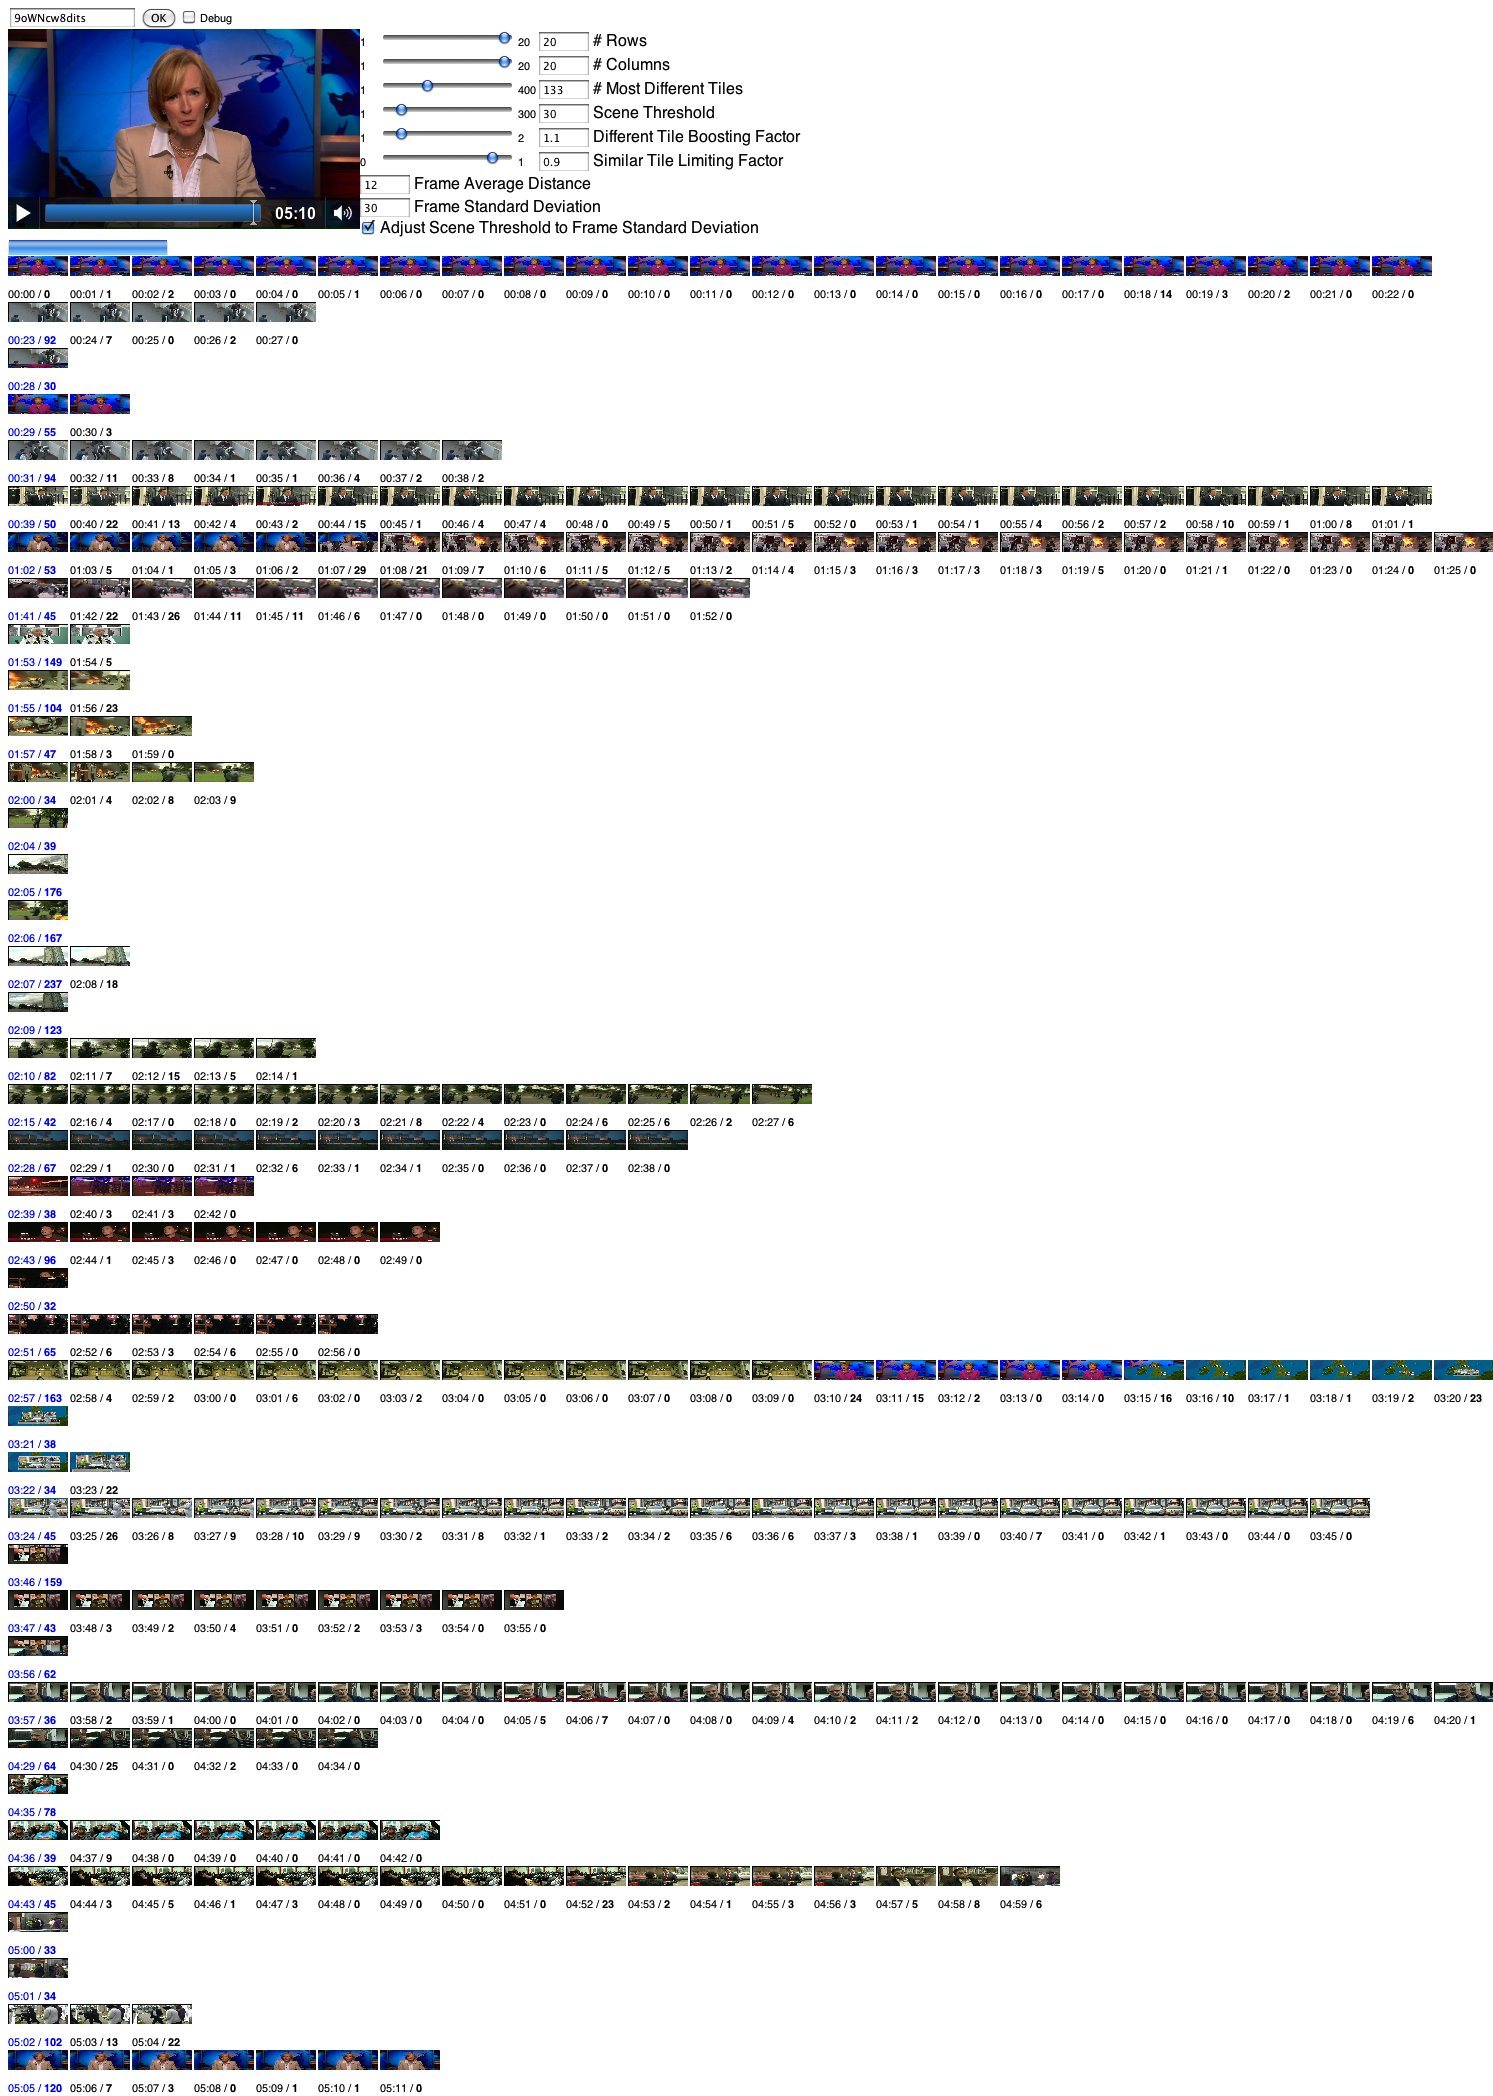
\includegraphics[width=0.7\linewidth]{./resources/london}
\end{center}
   \caption{Exemplary shots detected in a YouTube video on the London riots.}
\label{fig:shots}
\end{figure}
\end{comment}

\paragraph{Occurrences Event Detection Process}
In~\cite{semwebvid}, we document an interactive Web application that allows for the automatic annotation of videos on YouTube in RDF based on title, description, tags, and closed captions. In the current implementation we use \texttt{Factor}, \texttt{Product}, and \texttt{Agent} from the Event Ontology~\cite{Raimond:Event} to relate events to factors (everything used as a factor in an event), products (everything produced by an event), and agents (everything that can serve as an event agent). \autoref{code:semwebvid} shows a sample video fragment annotated with the Event Ontology.

\begin{lstlisting}[caption=Exemplary extracted named entities from a YouTube video on the London riots., label=code:semwebvid, float=htb!, escapechar=§]
<http://gdata.youtube.com/[...]/9oWNcw8dits> event:Event :event .

:event
  a event:Event;
  event:time [
    tl:start "PT0.00918S"^^xsd:duration;
    tl:end "PT0.01459S"^^xsd:duration;
    tl:duration "PT0.00541S"^^xsd:duration;
    tl:timeline :timeline;
  ];
  event:factor <http://dbpedia.org/resource/David_Cameron>;
  event:factor <http://sw.opencyc.org/2008/06/10/concept/en/§\linewrap§
      PrimeMinister_HeadOfGovernment>;
  event:factor <http://dbpedia.org/resource/Plastic_bullet>;
  event:factor <http://dbpedia.org/resource/Water_cannon>;
  event:product [
    a bibo:Quote;
    rdf:value """Prime Minister David Cameron authorized police
              to use plastic bullets and water cannons,"""@en;
  ] .
\end{lstlisting} 

\paragraph{Interest-based Event Detection Process}
For each scene in a video, we generate a set of \texttt{<img>} elements. These sets get injected into the YouTube homepage's DOM tree, as can be seen in \autoref{fig:youtube}. Each of the \texttt{<img>} elements has a registered JavaScript event handler that upon click triggers two actions: first, the video seeks to the corresponding time, and second, the shot is tracked as a point of interest in the video. We therefore use Google Analytics event tracking~\cite{analyticsevent}, logging the video ID and the video timestamp.

\subsection{Bringing It All Together}
From a Linked Data~\cite{Hausenblas:LDOW09} point of view, the main challenge with our browser extension was to decide on an as-consistent-as-possible way to model the three different event types of \emph{visual events}, \emph{occurrence events}, and \emph{interest-based events}. We decided for a combination of two vocabularies: the Event Ontology~\cite{Raimond:Event} mentioned before, and the W3C Ontology for Media Resources~\cite{mediaontology}, which aims to foster the interoperability among various kinds of metadata formats currently used to describe media resources on the Web. This ontology allows for the definition of media fragments. For this purpose we follow the Media Fragments URIs~\cite{W3C:MediaFrags} W3C Working Draft that specifies the syntax for media fragment URIs along several dimensions. The temporal dimension denotes a specific time range in the original media denoted by the~\texttt{t} parameter. In our case, a media fragment is the part of a video spun by the boundaries of the shot that contains the frame that the user clicked. \autoref{code:combined} shows an exemplary semantic annotation of a 27s long video shot containing a \emph{visual event} (the shot itself), an \emph{occurrence event} (the DBpedia URI representing David Cameron), and an \emph{interest-based event} (a point of interest spanning the whole shot). 

\begin{lstlisting}[caption=Semantic annotation of a 27s long video shot (\emph{visual event}) showing David Cameron (\emph{occurrence event}) talk about the London riots. The shot is also a point of interest generated by a click of a YouTube user (\emph{interest-based event})., label=code:combined, float=htb!, escapechar=§]
<http://gdata.youtube.com/[...]/9oWNcw8dits> event:Event :event1.

:event1 a event:Event;
  event:time [
    tl:start "PT0.025269S"^^xsd:duration;
    tl:end "PT0.05305S"^^xsd:duration;
    tl:timeline :timeline;
  ];
  event:factor <http://dbpedia.org/resource/David_Cameron>;
  event:product [
    a bibo:Quote;
    rdf:value """on camera. DAVID CAMERON, British prime
              minister: We needed a fight back, and a fight
              back is under way. [...] there are things that
              are badly wrong in our society. [...]"""@en;
  ];
  event:product §\linewrap§
      <http://gdata.youtube.com/[...]/9oWNcw8dits#t=25,53>.
      
<http://gdata.youtube.com/[...]/9oWNcw8dits#T=25,53> a §\linewrap§
    ma:MediaFragment.
\end{lstlisting} 

\section{Discussion of Our Approach}
Regarded in isolation, neither of our video event analysis steps is new, as detailed in~\autoref{sec:related-work}. We see our contributions (i) in the scalability through crowdsourcing, (ii) in the on-the-fly HTML5 client-side nature of our approach, and (iii) in the combination of the three different event type annotations. Hence, we discuss our preliminary results in contrast to a classic centralized approach. For \emph{visual event} analysis, rather than detecting shots client-side with HTML5 JavaScript APIs, a centralized approach with low level video tools is superior in terms of accuracy and speed, as the video files do not have to be streamed before they can be processed. In terms of scalability, however, the crowdsourced approach is superior. For \emph{textual event} detection, this is a task that necessarily runs centrally and not at the client due to the required huge text corpora. Finally, \emph{behavioral event} detection by definition is only possible on the client. While most users are not aware that their navigation behavior can be used to detect points of interest and thus behave naturally, fraud detection is necessary to filter out pseudo navigation events from spammers. 

\begin{comment}
% TOM: what is the best option to force linebreaks in a table cell? This boxing thing looks just plain wrong.
\begin{table}
\begin{center}  
    \begin{tabular}{ | l | c | c |}
    \hline
    \textbf{Event Type} & \textbf{Client-Side} & \textbf{Server-Side} \\ \hline
    \emph{Visual Event} & (+) More scalable (-) Streaming issues, slower & (+) Direct file access, faster (-) Less scalable \\ \hline
    \emph{Textual Event} & N/A & (+) Direct file access, faster (-) Limited scalability \\ \hline
    \emph{Behavioral Event} & (+) Scalable (-) Peril of spam & N/A \\ \hline
    \end{tabular}
\end{center}
\caption{Comparison of server-side and client-side video event detection.}
\label{table:comparison}
\end{table}
\end{comment}

\section{Future Work and Conclusion} \label{sec:future-work-conclusion}
\begin{comment}
In this paper, we have motivated why videos profit from richer crowd-generated event metadata and therefore have defined three different event types. We have shown related work in different fields and discussed crowdsourcing specifically in the context of video annotation. In continuation, we have described the implementation details of a browser extension for crowdsourced event detection and evaluated our crowdsourced approach against a classic server-based approach.
\end{comment}

Future work will focus on several aspects. First, given the streaming video nature, our approach inherits the speed and accuracy challenges from~\cite{artemis}; the solution here is to work with lower resolution versions of the video files in the background. Second, more elaborate interaction tracking for \emph{interest-based events} is necessary. Facets like playing time after a navigational click can shine more light on the quality of the believed point of interest. If a user clicks on a supposedly interesting scene, however, navigates away quickly afterwards, this is a strong indicator we need to consider. In the complete opposite, if a user never navigates within a video, this can be an indicator that the video is exciting from the first second to the last. Third, rather than just enriching the user experience for the current video, we will explore in how far the crowd-generated background knowledge gained on videos can be used for a more efficient video recommender system. This can be evaluated via A/B blind tests on clickthrough rates, where a user is randomly presented with a YouTube-generated related video recommendation, and a recommendation generated by the browser extension. 

 Concluding, our crowdsourced approach has shown promising results. The combination of \emph{textual}, \emph{visual}, and \emph{behavioral} analysis techniques provides for high quality metadata that otherwise could only be generated through human annotators. Our framework is a scalable first step towards video event detection, with actionable steps ahead.

% back to normal size Computer Modern for URLs in bibliography
\renewcommand{\ttdefault}{cmvtt}
\renewcommand\UrlFont\tt

\bibliographystyle{splncs03}
\bibliography{derive2011}

\end{document}